\chapter{协议设计}

\section{源文件架构}

\begin{figure}[htbp!]
    \centering
    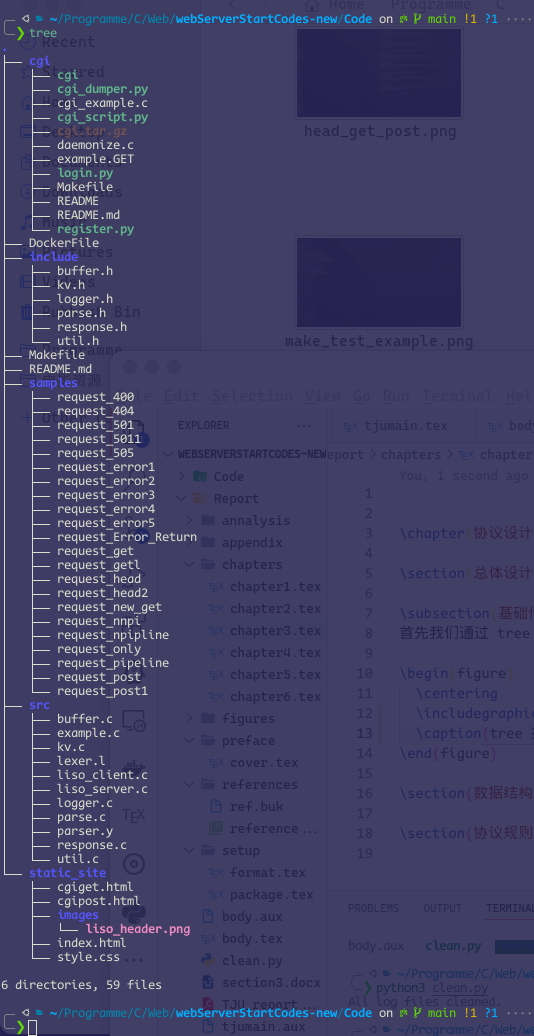
\includegraphics[width=5.5in]{Web_code_Structure.png}
    \caption{Structure of the Source Code}\label{fig:Web_code_structure}
    \vspace{-1em}
\end{figure}

如图\ref{fig:Web_code_structure}所示,源文件由$cgi$, $include$, $samples$, $src$ 和 $static\_sites$ 五个文件夹和 $Makefile$ 组成,其中 $include$,$src$,$samples$ 和 $Makefile$ 是第一周实验需要用到的文件。

\begin{itemize}
    \item include 文件夹中包含一个 parse.h 文件,是用于解析报文的 parse.c 文件的头文件,其中定义了重要的结构体 Request\_header 和 Request,并给出了共 echo\_server 和 echo\_client 调用的解析接口 Request* parse(char *buffer, int size,int socketFd)。(截图中的文件 util.h 是方便调试写进去的工具包:包括一些方便输出的宏定义);

    \item src 文件夹中包含三组代码:负责消息解析的 parser.y,parse.c,和lexer.l;负责测试消息解析的 example.c 以及一个网络应用程序 echo\_client.c 和 echo\_server.c;
    
    \item samples 文件夹中包含各类消息,用于对消息解析的测试;
    
    \item Makefile 负责管理项目的编辑。

\end{itemize}


\section{功能模块}

基础代码的功能主要包括两大部分:
\begin{enumerate}
    \item 测试 parcer 解析的情况:由 parse.c, parser.y 等文件组成,用于调试
    \item 网络应用程序,即使用 socket 进行通信的 echo\_server 和 echo\_client 两个文件
\end{enumerate}

\section{消息解析}

消息解析中,采用的是 yacc 和 lex 相配合的方式,二者的关系可以由图\ref{fig:yaccLex}指出,即 Lex 用于分词,Yacc 用于语义的翻译。

\begin{figure}[htbp!]
    \centering
    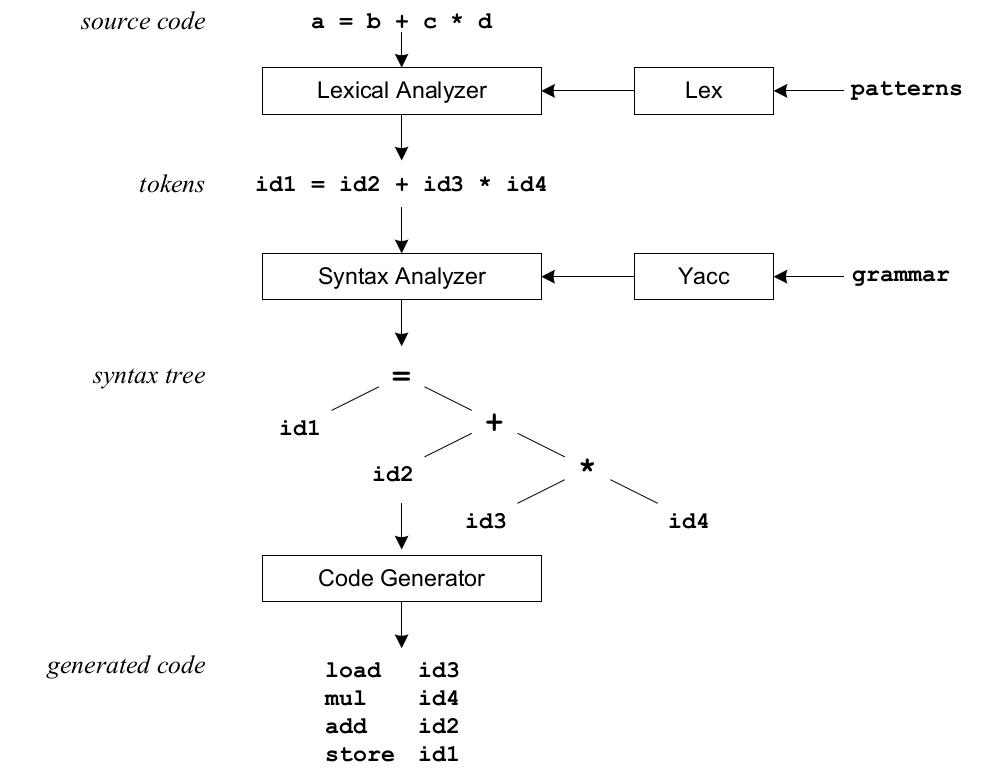
\includegraphics[width=4.5in]{yaccLex.png}
    \caption{Yacc and Lex}\label{fig:yaccLex}
    \vspace{-1em}
\end{figure}

具体到代码层面,我们主要关注 parser.y,即 Yacc 部分。我们需要通过添加更多的 grammar 和 相关的操作,来解析更多消息的类型。


